% ****** Start of file apssamp.tex ******
%
%   This file is part of the APS files in the REVTeX 4.1 distribution.
%   Version 4.1r of REVTeX, August 2010
%
%   Copyright (c) 2009, 2010 The American Physical Society.
%
%   See the REVTeX 4 README file for restrictions and more information.
%
% TeX'ing this file requires that you have AMS-LaTeX 2.0 installed
% as well as the rest of the prerequisites for REVTeX 4.1
%
% See the REVTeX 4 README file
% It also requires running BibTeX. The commands are as follows:
%
%  1)  latex apssamp.tex
%  2)  bibtex apssamp
%  3)  latex apssamp.tex
%  4)  latex apssamp.tex
%
\RequirePackage{lineno}
\setlength{\linenumbersep}{6pt}

\documentclass[%
reprint,
%superscriptaddress,
%groupedaddress,
%unsortedaddress,
%runinaddress,
%frontmatterverbose, 
%preprint,
showpacs,preprintnumbers,
%nofootinbib,
%nobibnotes,
%bibnotes,
 amsmath,amssymb,
 aps,
%pra,
%prb,
%rmp,
%prstab,
%prstper,
%floatfix,
]{revtex4-1}

\usepackage{graphicx}% Include figure files
\usepackage{dcolumn}% Align table columns on decimal point
\usepackage{bm}% bold math
\usepackage{xspace}	% Include xspace
\usepackage{color}
\usepackage{xcolor}
\usepackage{amsmath}
%\usepackage{hyperref}% add hypertext capabilities
%\usepackage[mathlines]{lineno}% Enable numbering of text and display math
%\linenumbers\relax % Commence numbering lines

%\usepackage[showframe,%Uncomment any one of the following lines to test 
%%scale=0.7, marginratio={1:1, 2:3}, ignoreall,% default settings
%%text={7in,10in},centering,
%%margin=1.5in,
%%total={6.5in,8.75in}, top=1.2in, left=0.9in, includefoot,
%%height=10in,a5paper,hmargin={3cm,0.8in},
%]{geometry}

\newcommand{\pt}{\mbox{$p_T$}\xspace}
\newcommand{\raa}{\mbox{$R_{\rm AA}$}\xspace}
\newcommand{\raap}{\mbox{$R_{\rm AA}^{N_{\rm part}}$}\xspace}
\newcommand{\Npart}{\mbox{$N_{\rm part}$}\xspace}
\newcommand{\Ncoll}{\mbox{$N_{\rm coll}$}\xspace}
\newcommand{\Nch}{\mbox{$N_{\rm ch}$}\xspace}
\newcommand{\Et}{\mbox{${\rm E}_T$}\xspace}
\newcommand{\meanpt}{\mbox{$\langle p_T \rangle$}\xspace}
\newcommand{\meanet}{\mbox{$\langle {\rm E}_T \rangle$}\xspace}
\newcommand{\mNcoll}{\mbox{$\langle N_{\rm coll} \rangle$}\xspace}
\newcommand{\sqs}{\mbox{$\sqrt{s}$}\xspace}
\newcommand{\sqsn}{\mbox{$\sqrt{s_{_{NN}}}$}\xspace}
\newcommand{\dau}{\mbox{$d$+Au}\xspace}
\newcommand{\dpb}{\mbox{$d$+Pb}\xspace}
\newcommand{\pau}{\mbox{$p$+Au}\xspace}
\newcommand{\pal}{\mbox{$p$+Al}\xspace}
\newcommand{\hau}{\mbox{$^3\text{He}$+Au}\xspace}
\newcommand{\pp}{\mbox{$p$+$p$}\xspace}
\newcommand{\ppb}{\mbox{$p$+Pb}\xspace}
\newcommand{\pa}{\mbox{$p+A$}\xspace}
\newcommand{\rdau}{\mbox{$R_{dAu}$}\xspace}
\newcommand{\pda}{\mbox{$p(d)+A$}\xspace}
\newcommand{\rpda}{\mbox{$R_{p(d)+A}$}\xspace}
\newcommand{\bbceta}{\mbox{$3.0<|\eta|<3.9$}\xspace}

\bibliographystyle{unsrt}

\linenumbers

\begin{document}

\title{Measurement of Long-Range Angular Correlations and Azimuthal Anisotropies in High Multiplicity \pau Collisions at \sqsn = 200 GeV}% Force line breaks with \\

\author{Author list: Brant will insert later}

\date{\today}% It is always \today, today,
             %  but any date may be explicitly specified

\begin{abstract}
We present the first measurements of long-range azimuthal correlations and the transverse momentum dependence of elliptic flow $v_2$ in high-multiplicity central \pau collisions at \sqsn = 200 GeV. A comparison of these results with those previously measured in central \dau and \hau demonstrates the direct relation between $v_2$ and the initial eccentricity $\varepsilon_2$. Such an observation allows us to ascertain the role of the initial geometry as a major driver of the collective behavior observed in small systems, potentially precluding theoretical explanations based on momentum-space domain correlations. Good agreement is observed between the measured $v_2$ and hydrodynamic calculations for all systems. The set of measurements here presented provides the opportunity to leveraged the distinct intrinsic geometry of these systems to provide stringent constraints for the theoretical extraction of medium properties. 
\end{abstract}

\pacs{25.75.Dw}% PACS, the Physics and Astronomy
                             % Classification Scheme.
%\keywords{Suggested keywords}%Use showkeys class option if keyword
                              %display desired
\maketitle

The azimuthal momentum anisotropy of particle emission relative to the reaction plane of the collision, as quantified by the Fourier coefficients $v_n$ of the final state particle yield, has long been considered evidence for the formation of a strongly interacting, fluid-like quark-gluon plasma (QGP) in A+A collisions~\cite{Snellings:2011sz}. Viscous hydrodynamics supports a picture in which the initial spatial inhomogeneities and fluctuations in energy density are propagated into the final state as anisotropies in momentum space.  The success of this model~\cite{Luzum:2008cw} in describing various bulk observables of the QGP has lent credence to the notion of hydrodynamic flow as the main driver of the $v_{n}$ signal in this class of collisions.

However, recent analyses of \dau and \hau at \sqsn = 200 GeV~\cite{adare_measurement_2014,Adamczyk:2014fcx,PhysRevLett.115.142301} at the Relativistic Heavy-Ion Collider (RHIC), and \ppb at \sqsn = 5.02 TeV and $p+p$ at \sqsn = 7 and 13 TeV~\cite{alice_long_2013,atlas_observation_2012,cms_observation_2012,Khachatryan:2015lva,Aad:2015gqa} at the Large Hadron Collider (LHC) have demonstrated the existence of the same kind of azimuthal anisotropy signals commonly interpreted as evidence of collective behavior in larger systems. Notably, a feature known as \textit{the ridge} has been observed, consisting of a near-side (i.e., around $\Delta \phi = 0$) enhancement in the azimuthal two-particle correlation even when accounting for non-flow contributions. This results in substantial elliptic ($v_2$), and triangular ($v_3$) flow coefficients being measured in these systems.

Although these observations seem to support the idea of QGP formation in small systems, the applicability of viscous hydrodynamics has not been clearly established in this regime, since any QGP formed in small systems is not expected to exist long enough for final-state anisotropies to develop as a consequence of hydrodynamic flow. Thus, other explanations have been proposed, including initial state effects from glasma diagrams~\cite{dusling_azimuthal_2012} and partonic scattering in transport models~\cite{bzdak_elliptic_2014,ma_long-range_2014,Koop:2015wea}. A key experimental test to resolve the issue consists in varying the intrinsic initial geometry of the system, and hence of the ensuing QGP, to analyze the extent to which it carries into the final state~\cite{nagle_exploiting_2013}. 

The PHENIX collaboration has actively pursued this course of study by analyzing data from intrinsically elliptic (\dau)~\cite{adare_measurement_2014,PhysRevLett.111.212301} and triangular (\hau)~\cite{Adare:2015ctn} collision systems at \sqsn = 200 GeV. Viscous hydrodynamics has been found to accurately reproduce the measured $v_n$~\cite{Romatschke:2015gxa} for these systems, establishing the relevance of the initial geometry and hydrodynamic flow in the development of the $v_n$ signal in small systems.

This communication completes the above suite of studies by presenting two-particle correlations and the transverse momentum (\pt) dependence of $v_2$ for central \pau collisions at \sqsn = 200 GeV. These results are compared to those from \dau and \hau in the same centrality class, as well as to available theoretical calculations.

A detailed description of the PHENIX detector can be found in Ref.~\cite{Adcox2003469}. For this analysis, charged particles were reconstructed with the two central arm spectrometers, consisting of drift chambers (DC) and multi-wire proportional pad chambers (PC) covering $|\eta|<0.35$ and $\pi/2$ in azimuthal angle. Drift chamber tracks are matched to hits in the third layer of the PC, thus limiting the contribution of tracks from decays and photon conversions. The beam-beam counters (BBC) comprise two arrays of 64 quartz radiator \v{C}erenkov detectors, located longitudinally $\pm$1.44 m away from the center of the interaction region (IR), covering \bbceta and 2$\pi$ in azimuth. The FVTX is a silicon detector comprising two identical end-cap assemblies symmetrically located in the longitudinal direction around the IR, covering $1.0 < |\eta| < 3.0$. It uses hit clusters to detect charged particles with an efficiency of over 95\%. Relative to the PHENIX coordinate system, the Au-beam points southward in the direction of negative pseudorapidity. Hence, the arms of the BBC and FVTX in that direction are designated as the \emph{south} arms of the detectors, and styled as BBC-S and FVTX-S, respectively.
A $\pm$30 cm event vertex cut was applied for all analyses, corresponding to the acceptance of the central arms. 

%The event planes are measured in the Au-going direction using the south BBC (BBC-S) covering $−3.9 < \eta < −3.0$, as well as the reconstructed clusters in the south end-cap of FVTX (FVTX-S) covering $−3.0 < \eta < −1.0$.  

The \pau data set for this analysis was collected during the 2015 data-taking run at RHIC. It consists of 0.84 billion minimum bias (MB) triggered events and 1.4 billion high-multiplicity (HM) triggered events. The MB trigger is defined as a coincidence between the Au-going and $p$-going BBC detectors, requiring at least one photomultiplier tube (PMT) firing in each; in this way 84$\pm$4\% of the total inelastic \pau cross section is captured. The HM trigger is based on the MB trigger, but imposes the additional requirement of more than 48 photomultiplier tubes firing in the BBC-S. A description of the \dau and \hau data sets used in this analysis can be found in Refs.~\cite{adare_measurement_2014} and ~\cite{PhysRevLett.115.142301}, respectively. 

In this analysis, we select the 0-5\% most central \pau, \dau, and \hau events, where 
centrality classes are defined as a percentile of the total multiplicity measured in the BBC-S, following the procedure documented in Ref.~\cite{bbc}.
The initial geometry of events in these centrality selections is characterized using a standard Monte Carlo Glauber approach, where nucleon coordinates are smeared by a Gaussian profile of $\sigma = 0.4$ fm. The results of this characterization are shown in Table~\ref{table_geometry}, 

\begin{table}
\caption{Geometric characterization of small system collisions at \sqsn = 200 GeV in the 0-5\% centrality class, using Monte Carlo Glauber with nucleon coordinates smeared by a two-dimensional Gaussian of width $\sigma=0.4$ fm.}
\begin{ruledtabular}
\begin{tabular}{c c c c}
\label{table_geometry}
 & \pau (0-5\%) & \dau (0-5\%) & \hau (0-5\%) \\
\hline
 $\langle Q_{BBC} \rangle$ & 58.9 & ? & ? \\
 $\langle N_{coll} \rangle$ & $9.7\pm 0.6$ & $18.1\pm 1.2$ & $26.1\pm 2.0$ \\
 $\langle N_{part} \rangle$ & $10.7\pm 0.6$ & $17.8\pm 1.2$ & $25.1\pm  1.6$ \\ 
 $\langle \varepsilon_2 \rangle$ & $0.23\pm 0.01$ & $0.54\pm 0.04$ & $0.50\pm 0.02$ \\
 $\langle \varepsilon_3 \rangle$ & $0.16\pm 0.01$ & $0.19\pm 0.01$ & $0.28\pm 0.02$
\end{tabular}
\end{ruledtabular}
\end{table}

Long-range angular correlations are constructed between charged tracks in the PHENIX central arms at a given \pt, and charge deposited in the BBC-S PMTs, for central \pau collisions at \sqs~=~200~GeV. The distribution of these track-PMT pairs is constructed over relative azimuth, with the normalized correlation function given by Eq.~\ref{eq:def_corr_function}, following Ref.~\cite{PhysRevLett.115.142301}:
\begin{eqnarray}
  S(\Delta\phi,p_{T})=
  \frac{ d(w_{{\rm PMT}} N^{{\rm track}(p_{T}){\rm - PMT}}_{{\rm Same \; event}}) }{ d\Delta\phi}, & &
\label{eq31} \\
  C(\Delta\phi,p_{T}) =
          \frac{S(\Delta\phi,p_{T})}{M(\Delta\phi,p_{T})} \:
          \frac{\int_{0}^{2\pi} M(\Delta\phi,p_{T}) \, d\Delta\phi}{\int_{0}^{2\pi} S(\Delta\phi,p_{T}) \, d\Delta\phi}. & &
  \label{eq:def_corr_function}
\end{eqnarray}
The weights $w_{{\rm PMT}}$ for each pair correspond to the charge in the PMTs. The signal distribution $S$ is constructed from pairs in the same event. The mixed distribution $M$ is taken over pairs from different events in the same centrality class and $z$ vertex bin, to correct for non-uniformity in the acceptance over $\Delta \phi$.

%%%%%%%%%%%%%%%%%%%%%%%%%%%%  Fig_1 %%%%%%%%%%%%%%%%%%%%%%%%%
% figure showing BBC-S-CNT correlations
\begin{figure*}[htbp]
  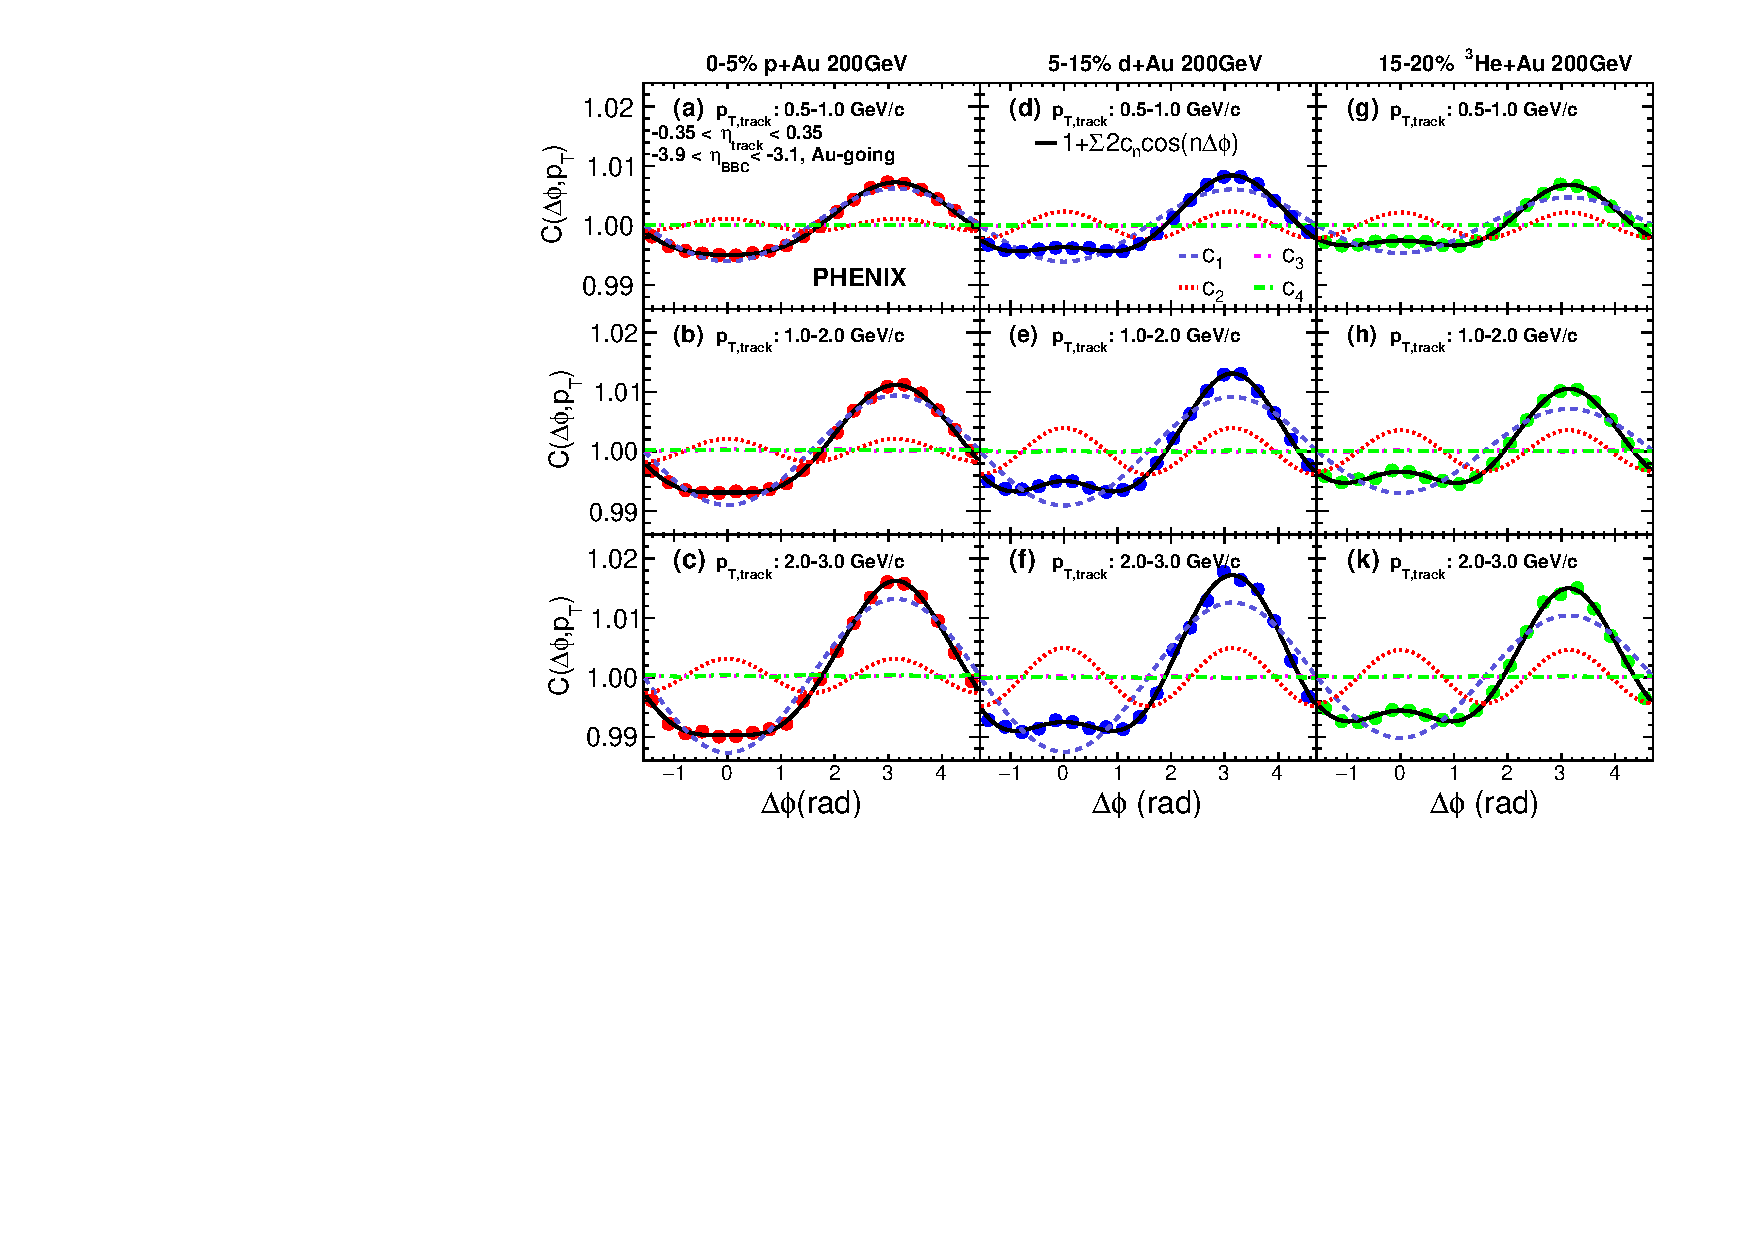
\includegraphics[scale=0.8]{Figures/figure1.pdf}
  \caption{(Color online) Long-range angular correlations $C(\Delta\phi,p_{T})$ constructed with central arm tracks and BBC-S PMT pairs, in 0\%--5\% central \pau collisions at \sqsn~=~200~GeV. From left to right,
correlations are shown for various track \pt selections: (a) 0.5--1.0 GeV/$c$, (b) 1.0--2.0 GeV/$c$, and (c) 2.0--3.0~GeV/$c$. We fit each correlation with a four-term Fourier cosine series; individual harmonics shown as dashed lines, and the total fit is shown as a solid line.}
\label{fig:figure1}
\end{figure*}

%%%%%%%%%%%%%%%%%%%%%%%%%%%%  Fig_2 %%%%%%%%%%%%%%%%%%%%%%%%%
% figure showing c2 coefficients
\begin{figure}[htbp]
  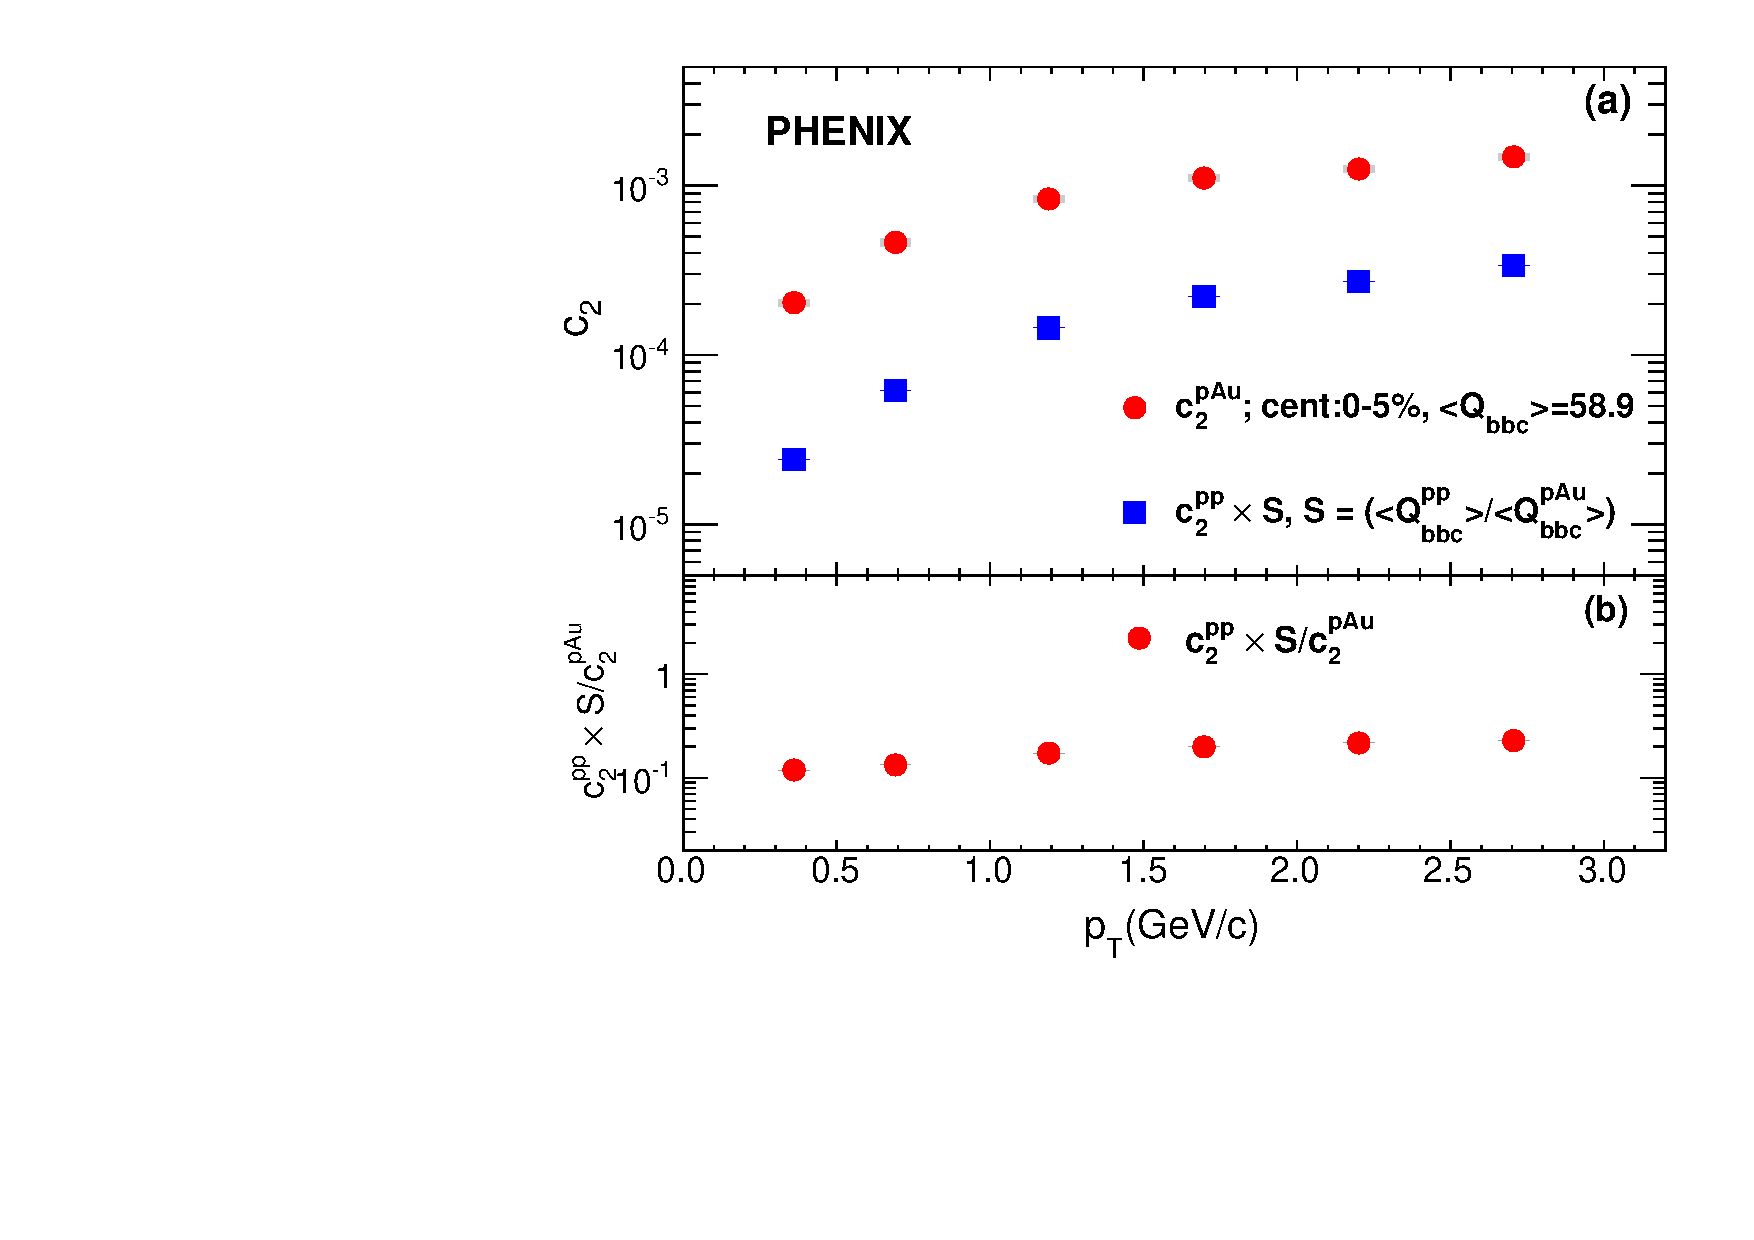
\includegraphics[scale=0.45]{Figures/figure2.pdf}
  \caption{(Color online)~The $c_2(p_T)$ coefficients for track-BBC pairs from 
0\%--5\% \pau, 5\%--15\% \dau and 10\%--15\% \hau collisions and
$c_{2}(p_{T})$ for pairs in minimum bias \pp collisions times the dilution
factor $\left( \sum Q^{{\rm BBC-S}} \right)_{p+p} / \left( \sum Q^{{\rm
BBC-S}} \right)_{{\rm pAu}}$ (open, denoted ``$c^{{\rm B}}$'' ). (b)~The
ratio $c^{{\rm B}}/c^{{\rm A}}$ is shown with statistical error bars.
}
\label{fig:figure2}
\end{figure}

The resulting correlation functions for a variety of central arm track \pt selections are shown in Figure ~\ref{fig:figure1}. Each one is fit with a four-term cosine Fourier series. The magnitude of the second harmonic ($c_{2}$) as a function of \pt is shown in red in panel (a) Fig.~\ref{fig:figure2}. The contribution of elementary processes (e.g., jet fragmentation) to the measured $c_2$ in \pau can be estimated quantitatively using the published $c_2$ from \pp at the same collision energy, yet scaled down by an appropriate factor to account for the greater number of binary nucleon collisions taking place in \pau. In this analysis, the scale factor is chosen to be the ratio of the total charge deposited in the BBC-s in \pp relative to \pau, as shown in Eq.~\ref{eq:dilute}. The scaled down \pp $c_{2}$ is shown in blue in panel (a) of Fig.~\ref{fig:figure2}. The ratio of $c_2$ in \pau to the scaled-down \pp reference is shown in panel (b). From this ratio, it can be seen that the relative correlation strength in \pau from elementary processes is at most 23\% at the highest \pt.

\begin{equation}
c_{n}^{{\rm pAu \; elementary}}(p_{T}) \simeq c_{n}^{p+p}(p_{T})
\frac{\left( \sum Q^{{\rm BBC-S}} \right)_{p+p}}
{\left( \sum Q^{{\rm BBC-S}} \right)_{{\rm pAu}}
}.
\label{eq:dilute}
\end{equation}

It is noteworthy that, unlike \dau~\cite{adare_measurement_2014} and \hau~\cite{PhysRevLett.115.142301} collisions at the same centrality, the long-range angular correlations in \pau do not exhibit a discernible near-side peak---suggesting a weaker collective behavior---yet possess a non-negligible second harmonic, as quantified by the measured $c_2(p_T)$. Additionally, it is observed that the relative contribution of elementary processes to the total correlation strength $c_2$ is much higher in \pau, being more than twice the value quoted for the other two systems using the same \pp reference. 

Having quantified the strength of elementary process contributions, we calculate the elliptic flow $v_2(p_T)$ using the event plane method, as described in Ref.~\cite{Adare:2015ctn}. Namely, we measure 

\begin{equation}
v_{2}(p_{T}) = \frac{\langle\sum \cos 2(\phi_{\text{Particle}}(p_{T})-\Psi^{\text{FVTX-S}}_{2})\rangle}{\text{Res}(\Psi^{\text{FVTX-S}}_{2})}
\end{equation}

for charged hadrons at midrapidity, where the second order event plane $\Psi^{FVTX-S}_{2}$ is determined for every event using the FVTX-S detector. Its resolution is computed using the standard three-subevent method, resulting in $\text{Res}(\Psi^{\text{FVTX-S}}_{2})$ = 0.171. It is also possible to measure the event plane using the BBC-S. In that case, we obtain a lower resolution $\text{Res}(\Psi^{\text{BBC-S}}_{2})$ = 0.062, and a $v_2$ that differs from the FVTX-S measurement by approximately 3\%.

\begin{eqnarray}
\text{Res}(\Psi^{FVTX-S}_n) &=& \langle \cos[n(\Psi^{BBC-S}_n - \Psi_{RP})] \rangle \\
&=& \sqrt{\frac{\langle \cos[n(\Psi^{BBC-S}_n - \Psi_{CNT})] \rangle \langle \cos[n(\Psi^{BBC-S}_n - \Psi^{FVTX-S}_n)] \rangle}{\langle \cos[n(\Psi^{CNT}_n - \Psi^{FVTX-S}_n)] \rangle}}
\end{eqnarray}
The main sources of systematic uncertainty on the $v_2(p_T)$ measurement are: (1) track background from photon conversion and weak decays, whose magnitude we estimate at 2\% by varying the spatial matching windows in the PC3 from 3$\sigma$ to 2$\sigma$; (2) multiple collisions per bunch crossing (i.e., event pile-up) estimated at 8\% and given an asymmetric uncertainty of $^{+0}_{-4}\%$, since their effect if to lower the $v_2$; (3) non-flow correlations from elementary processes that enhance the $v_2$, whose contribution we estimate from Fig.~\ref{fig:figure2} as reaching a maximum of 23\% at the highest \pt; hence, we assign a $^{+0}_{-23}\%$ asymmetric uncertainty. (4) the azimuthal asymmetry between the east ($-\pi/2 < \phi < \pi/2$) and west ($\pi/2 < \phi < 3\pi/2$) acceptance of the detectors due to a misalignment of 3.6 mrad between the colliding beams and the longitudinal axis of PHENIX. We applied a corresponding counter-rotation to every central arm track and detector element in the FVTX and BBC, which were also reweighted to restore their uniformity in azimuth. We estimate this systematic uncertainty at 5\% by taking the difference of $v_2$ as measured independently in each detector arm after applying the above corrections. 

\label{s:sys}
%%%%%%%%%%%%%%%%%%%%%%%%%%%%%%%% Systematic Table %%%%%%%%%%%%%%%%%%%%%%%%%%%%%%%%%%%%
\begin{table}[htbp]
  \begin{center}
    \begin{tabular}{ccc}
      \hline
      \hline
      Error Sources& systematic error & Type \\ \hline
      Event-plane detectors & 3\% & A\\
      Background &2.0\%& A\\
      Pile up    &$^{+0}_{-4}\%$& B\\
      nonflow    &$^{+0}_{-23}\%$& B\\
      Acceptance &5.0\%& C\\
    \hline
    \hline
    \end{tabular}
   \caption{\label{t:sys}Systematic uncertainties given in percent on the $v_2$ measurements.}
   \end{center}
 \end{table}

Table~\ref{t:sys} summarizes of all these systematic
uncertainties, which are categorized by type:

(A) point-to-point error uncorrelated between $p_T$ bins,

(B) $p_{T}$-correlated, all points move in the same direction but
not by the same amount,

(C) an overall normalization error in which all points move by the
same amount, independently of $p_T$.

The resulting $v_2$ measurement for \pau, compared to \dau and \hau in the same centrality, is shown in Fig.~\ref{fig:figure3}. The possibility of comparing the final state particle emission patterns---as quantified by $v_2$---of three collision systems with intrinsically different projectile geometry provides a valuable opportunity to quantitatively study the effect of initial geometry in the development of collectivity.  In all cases, there is a substantial $v_2$ that rises with \pt. The ordering of the curves directly correlates with the ordering of initial eccentricities $\varepsilon_2$, as presented in Table~\ref{table_geometry}. Namely, \dau has the highest $\varepsilon_2$, but close to that of \hau, while \pau has a much lower $\varepsilon_2$ than the other two systems. These results are consistent with a physical picture of small systems where initial geometry is the driver of final-state momentum anisotropy.

To further test this idea, we divide the $v_2$ curves by their corresponding $\varepsilon_2$ from Table~\ref{table_geometry}, attempting to establish a scaling relation between these two quantities. Unlike the case of ideal hydrodynamics in A+A, the ratios do not collapse to a common value, as shown in Figure~\ref{fig:figure4}. This imperfect scaling should not be interpreted as suggesting that the nature of small system collectivity is fundamentally different from that in A+A. Instead, it can be understood in terms of a \emph{short lived} QGP, expanding hydrodynamically just as in larger systems, yet unable to translate the initial geometry into the final-state in events with a limited number of hot spots far apart from each other, as discussed in Ref.~\cite{nagle_exploiting_2013}.

\begin{figure}[htbp]
  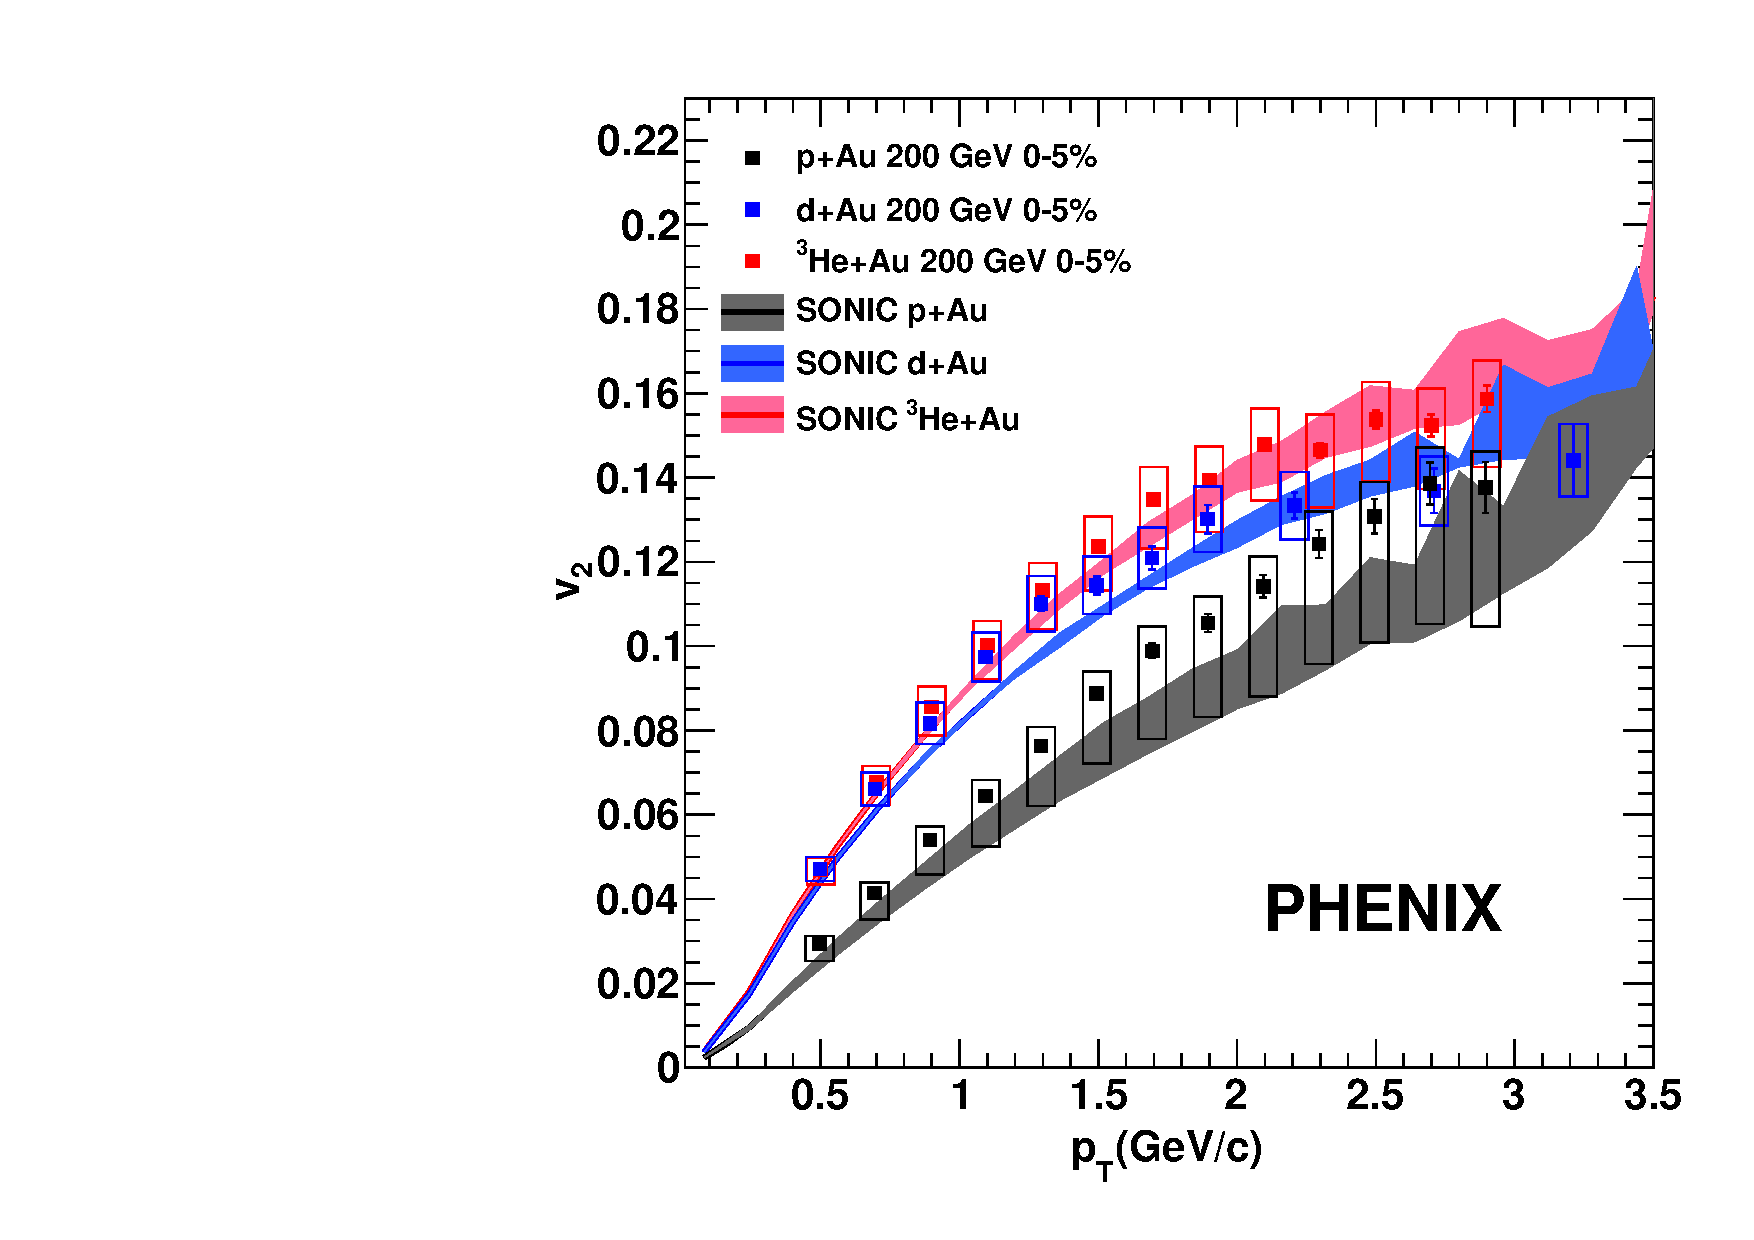
\includegraphics[scale=0.45]{Figures/figure3.pdf}
  \caption{(Color online)$v_2$ of charged hadrons within $|\eta| <$ 0.35 in 0\%--5\% \pau, \dau, and \hau collision.}
\label{fig:figure3}
\end{figure}

\begin{figure}[htbp]
  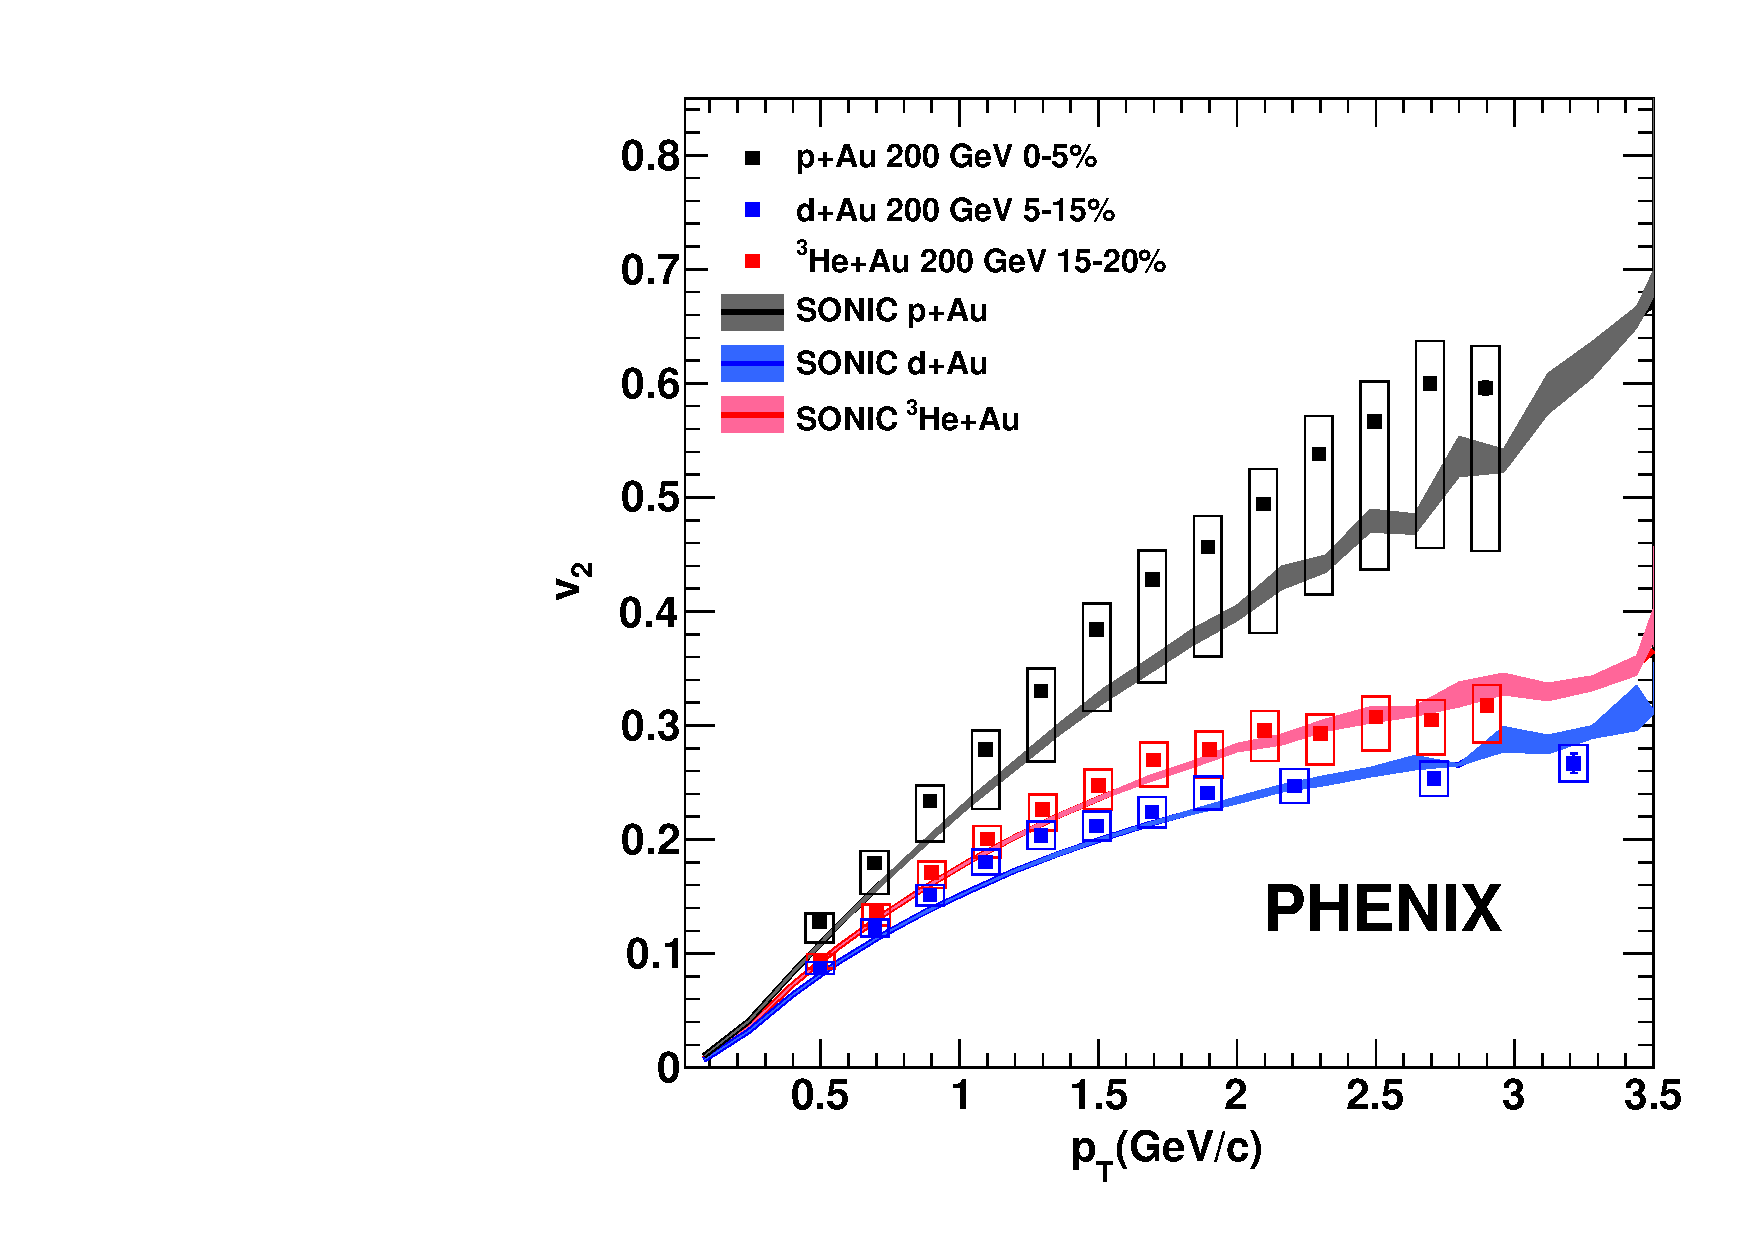
\includegraphics[scale=0.45]{Figures/figure4.pdf}
  \caption{(Color online)$v_2$ of charged hadrons within $|\eta| <$ 0.35 in 0\%--5\% \pau, \dau and \hau collisions, divided by their corresponding eccentricity $\varepsilon_2$ from Glauber calculations.}
\label{fig:figure4}
\end{figure}

%%%%%%  Main figure with final results and theory curves
%%%give this part to Javier for theory comparisons
In addition to confirming the importance of initial geometry, the results in Figure~\ref{fig:figure3} and their imperfect geometric scaling provide a stringent test for any theoretical model attempting to describe small system collectivity. Figure~\ref{fig:figure5} shows $v_2(\pt)$ for 0-5\% central \pau, \dau, and \hau events, for which theoretical predictions are available in the literature, most notably from hydrodynamics with Glauber initial conditions (\textsc{sonic}~\cite{Habich:2014jna} and \textsc{supersonic}~\cite{Romatschke:2015gxa}), hydrodynamics with IP-Glasma initial conditions~\cite{Schenke:2014gaa}, and A-Multi-Phase-Transport Model (\textsc{ampt})~\cite{lin_multiphase_2005}.

\begin{figure*}[htbp]
  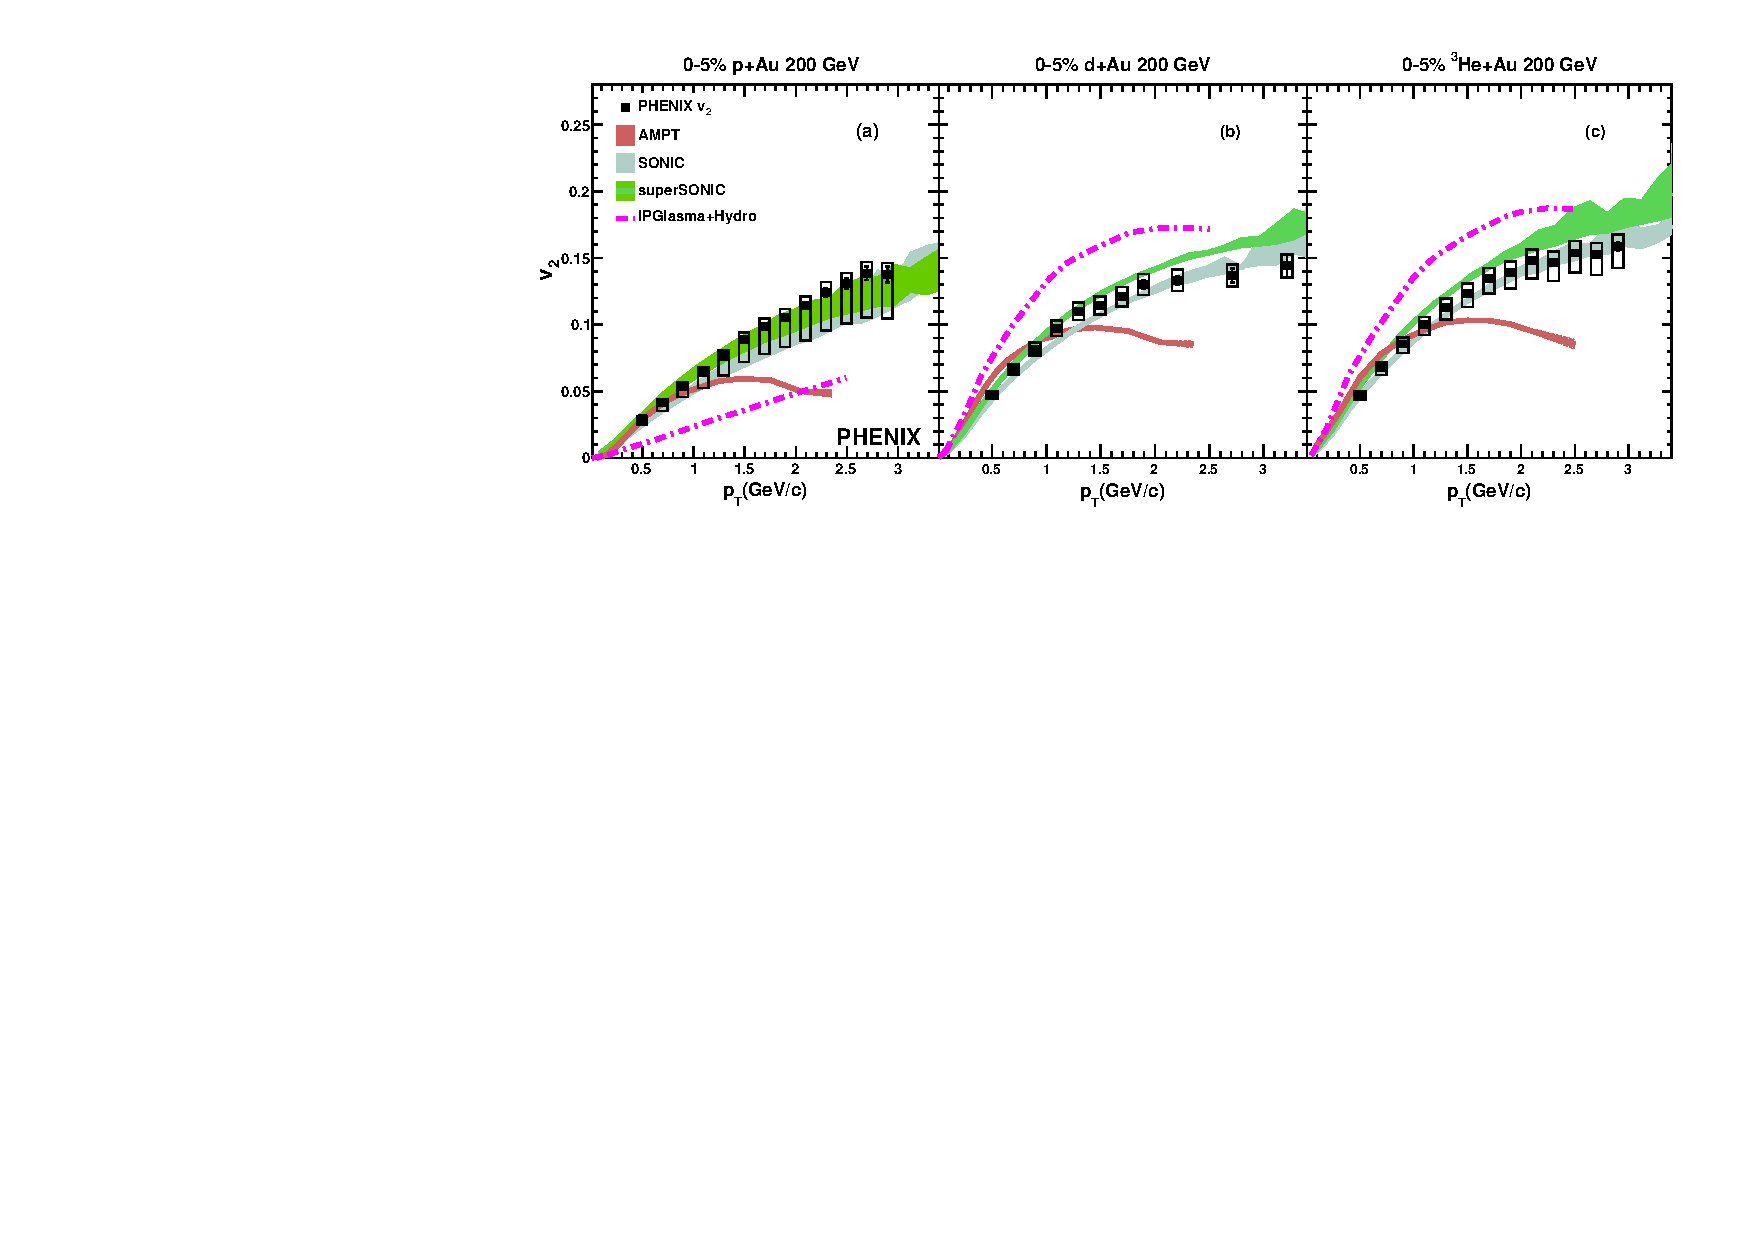
\includegraphics[scale=0.9]{Figures/figure5.pdf}
  \caption{(Color online) Transverse momentum dependence of $v_2$ in central 0-5\% (a) \pau, (b) \dau, and (c) \hau collisions at \sqsn = 200 GeV. Theoretical calculations from \textsc{ampt}, \textsc{(super)sonic}, and IPGlasma+Hydro are shown in each panel.}
%%Results for $v_{2}$ (circles) and $v_{3}$ (squares) as a function of \pt
%%for inclusive charged hadrons at mid-rapidity in 0\%--5\% central \heau
%%collisions at \sqsn~=~200~GeV; error bars are statistical and shaded bars
%%are systematic uncertainties as described in the text. Also shown are
%%various theoretical calculations, see text for details and references.}
\label{fig:figure5}
\end{figure*}

\begin{table}
\caption{Geometric characterization of small systems at \sqsn = 200 GeV for 0-5\% centrality from IP-Glasma initial conditions, and Monte Carlo Glauber initial conditions smeared with a two-dimensional Gaussian of width $\sigma=0.4$ fm.}
\begin{ruledtabular}
\begin{tabular}{c c c c}
\label{table_geometry_glasma}
 & \pau & \dau & \hau \\ \hline
 Glauber $\langle \varepsilon_2 \rangle$ & $0.231\pm 0.010$ & $0.540\pm 0.040$ & $0.504\pm 0.020$ \\
 IP-Glasma $\langle \varepsilon_2 \rangle$ & $0.099\pm 0.022$ & $0.595\pm 0.009$ & $0.555\pm 0.008$ \\
\end{tabular}
\end{ruledtabular}
\end{table}

The \textsc{sonic} and \textsc{supersonic} models incorporate standard Monte Carlo Glauber initial conditions followed by viscous hydrodynamics, and a transition to a hadronic cascade at T = 170 MeV. Furthermore, \textsc{supersonic} incorporates pre-equilibrium dynamics with a calculation in the framework of the AdS/CFT correspondence~\cite{vanderSchee:2013pia,Chesler:2015wra,Romatschke:2013re}. These two models agree well with the data within uncertainties, supporting the idea of initial geometry as the driver of the $v_n$ signal. Furthermore, this illustrates how these results impose useful constraints to reduce the number of \emph{free parameters} of the model, since many such parameters must be identical across systems, e.g., $\eta/s$, the transition temperature to a hadron cascade, and the nucleon cross section of $\sigma=0.4$ fm.

Predictions using IP-Glasma initial conditions followed by viscous hydrodynamics substantially overestimate the data for \dau and \hau, while underestimating it for \pau. This follows from the fact that IP-Glasma generates very \emph{circular} initial conditions for \pau, corresponding to very low $\varepsilon_2$ values; however, the presence of several hot spots in \dau and \hau result in IP-Glasma values for $\varepsilon_2$ more comparable to those from Glauber. This is shown in Table~\ref{table_geometry_glasma}. In the case of \dau and \hau, a better agreement with data can be achieved by increasing the value of $\eta$/s or by including a hadronic cascade stage. However, doing so would lower the prediction for \pau even further. This demonstrates that IP-Glasma does not generate the appropriate initial conditions to account for measured $v_n$ via hydrodynamic flow. 

It is important to notice that additional degrees of freedom on the geometry of \pau collisions arise from $x-$dependent fluctuations of the shape of the proton, as described in Ref.~\cite{Schlichting:2014ipa}. The contribution of this effect to the measured elliptic flow must be constrained by $p+p$ data, and also possibly by varying the target in other $p+$A systems.

Finally, \textsc{ampt} combines partonic and hadronic scattering in a single model. Using the initial Glauber geometry information to compute $v_2$ relative to the participant plane~\cite{Koop:2015wea} yields results that agree reasonably well with the data below $\pt \approx 1$ GeV/c, yet underpredict them at higher \pt. It is noteworthy that despite the very different physics of \textsc{ampt} compared to the other models, it has successfully been applied to a variety of systems at RHIC~\cite{Adare:2015cpn,Koop:2015wea}, and small systems at the LHC~\cite{ma_long-range_2014,ma_long-range_2014}.

We have presented results on azimuthal anisotropies and elliptic flow in central \pau at \sqsn = 200 GeV, compared with $v_2$ in \dau and \hau. These results impose strong constraints on models attempting to describe the formation and behavior of hot nuclear matter in small systems. We observe a clear---albeit imperfect---scaling of $v_2$ with $\varepsilon_2$, providing strong evidence for initial geometry as the source of final-state momentum anisotropies in these systems. This potentially precludes other explanations based on initial-state momentum space domain effects. Calculations from \textsc{sonic} and \textsc{supersonic} are able to reproduce the measured $v_2$ and their scaling behavior for central events in all systems, thus establishing hydrodynamics as a valid model to understand the physics of collectivity in this regime. 

\bibliography{references}
\end{document}
%
% ****** End of file apssamp.tex ******